% coding:utf-8

%----------------------------------------
%FOSAMATH, a LaTeX-Code for a mathematical summary for basic analysis
%Copyright (C) 2013, Daniel Winz, Ervin Mazlagic, Adrian Imboden, Philipp Langer

%This program is free software; you can redistribute it and/or
%modify it under the terms of the GNU General Public License
%as published by the Free Software Foundation; either version 2
%of the License, or (at your option) any later version.

%This program is distributed in the hope that it will be useful,
%but WITHOUT ANY WARRANTY; without even the implied warranty of
%MERCHANTABILITY or FITNESS FOR A PARTICULAR PURPOSE.  See the
%GNU General Public License for more details.
%----------------------------------------

% coding:utf-8
\section{Definition komplexe Zahlen}
Eine komplexe Zahl ist ein Vektor mit einer Komponente im realen Teil und 
einer Komponente im imaginären Teil. 

\section{Darstellung von komplexen Zahlen}
\subsection{Gausssche Zahlenebene}
Komplexe Zahlen können nicht auf dem Zahlenstrahl abgebilder werden. Daher wird 
dafür die gausssche Zahlenebene eingeführt. Das ist ein Koordinatensystem. Auf 
der x-Achse liegt der normale Zahlenstrahl. Auf der y-Achse wird die imaginäre 
Achse gelegt. 
\begin{center}
\begin{tikzpicture}[domain=-4:4]
  % Raster
  \draw[very thin,color=gray] (-1.9,-0.9) grid (3.9,2.9);
  % x-Achse
  \draw[->] (-2.2,0) -- (4.2,0) node[right] {$Re$};
  % y-Achse
  \draw[->] (0,-1.2) -- (0,3.2) node[above] {$Im$};
  % Linien, Pfeile
  \draw[-latex] (0,0) -- (3,2) node[right] {$a+bj$};
  \draw[-latex] (3,0) -- (3,2);
  \draw[-latex] (0,2) -- (3,2);
  % unabhängige Beschriftungen
  \node at (1.5,2.2) {a};
  \node at (3.2,1) {b};
  % Funktionen
%   \draw[color=red] plot (\x,0.5*\x) node[right] {$f(x) =0.5x$};
%   \draw[color=blue] plot (\x,{sin(\x r)}) node[right] {$f(x) = \sin x$};
%   \draw[color=orange] plot (\x,{0.05*exp(\x)}) node[right] {$f(x) = \frac{1}{20} \mathrm e^x$};
\end{tikzpicture}
\end{center}
Eine komplexe Zahl wird dabei in der Form $a+bj$ dargestellt, wobei 
$a, b \in \mathbb{R}$. 
\[ z = \text{Re} + j \cdot \text{Im} \]
\newpage

\subsection{Polardarstellung}
Bei der Polardarstellung wird eine Komplexe Zahl nicht mehr mittels der realen 
und imaginären Komponenten dargestellt. Stattdessen wird die Position der Zahl 
in der gaussschen Zahlenebene durch den Abstand vom Nullpunkt und den Winkel 
gegenüber der Horizontalen definiert. 
\begin{center}
\begin{tikzpicture}[domain=-4:4]
  % Raster
  \draw[very thin,color=gray] (-1.9,-0.9) grid (3.9,2.9);
  % x-Achse
  \draw[->] (-2.2,0) -- (4.2,0) node[right] {$Re$};
  % y-Achse
  \draw[->] (0,-1.2) -- (0,3.2) node[above] {$Im$};
  % Linien, Pfeile
  \draw[-latex] (0,0) -- (3,2) node[right] {$r \cdot \cis(\varphi)$};
  \draw[-latex] (1,0) arc (0:33.7:1);
  % unabhängige Beschriftungen
  \node at (1.2,0.3) {$\varphi$};
  \node at (1.5,1.3) {$r$};
  % Funktionen
%   \draw[color=red] plot (\x,0.5*\x) node[right] {$f(x) =0.5x$};
%   \draw[color=blue] plot (\x,{sin(\x r)}) node[right] {$f(x) = \sin x$};
%   \draw[color=orange] plot (\x,{0.05*exp(\x)}) node[right] {$f(x) = \frac{1}{20} \mathrm e^x$};
\end{tikzpicture}
\end{center}
\[ \boxed{z = r \cdot \cos(\varphi) + r \cdot j \cdot \sin(\varphi) 
= r \cdot \cis(\varphi)} \]

\subsubsection{Umrechnung Kartesisch $\rightarrow$ Polar}
\[ \boxed{r = \sqrt{x^2 + y^2}} \]
\[ \boxed{\varphi = \arctan{\left(\frac{y}{x}\right)}} \]

\subsubsection{Umrechnung Polar $\rightarrow$ Kartesisch}
\[ \boxed{x = r \cdot \cos(\varphi)} \]
\[ \boxed{y = r \cdot \sin(\varphi)} \]
\newpage

\subsection{Exponentialform}
\[ \boxed{z = r \cdot e^{j \varphi} \qquad , r = |z| \geq 0
, -\pi < \varphi \leq \pi, \varphi\text{ im Bogenmass}} \]

\subsubsection{Eulersche Formel}
\[ \boxed{e^{j \varphi} = \cos(\varphi) + j \cdot \sin(\varphi)} \]
\[ \boxed{e^{j \pi} + 1 = 0} \]

\subsection{Konjugiert komplex}
Der konjugiert komplexe Wert einer komplexen Zahl wird durch das Spiegeln an 
der x-Achse erreicht. 
\[ \boxed{\overline{a + b j} = a - b j} \]
\[ \boxed{\overline{r \cdot \cis(\varphi)} = r \cdot \cis(-\varphi)} \]
\[ \boxed{\overline{r \cdot e^{j \varphi}} = r \cdot e^{-j \varphi}} \]
\begin{center}
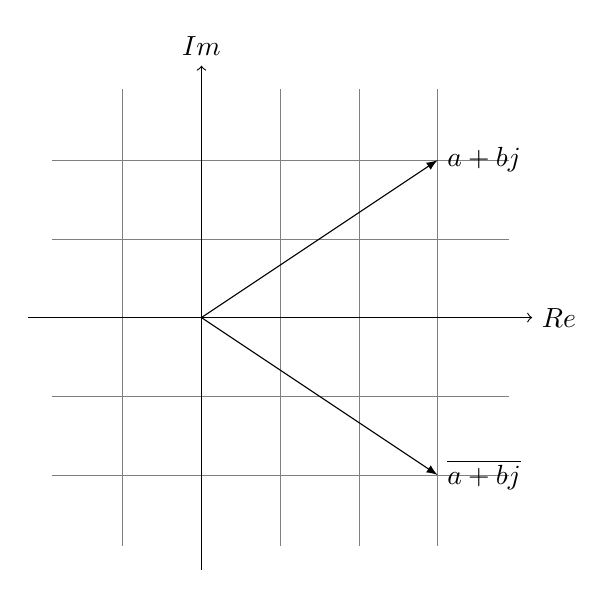
\begin{tikzpicture}[domain=-4:4]
  % Raster
  \draw[very thin,color=gray] (-1.9,-2.9) grid (3.9,2.9);
  % x-Achse
  \draw[->] (-2.2,0) -- (4.2,0) node[right] {$Re$};
  % y-Achse
  \draw[->] (0,-3.2) -- (0,3.2) node[above] {$Im$};
  % Linien, Pfeile
  \draw[-latex] (0,0) -- (3,2) node[right] {$a+bj$};
  \draw[-latex] (0,0) -- (3,-2) node[right] {$\overline{a+bj}$};
%   \draw[-latex] (0,2) -- (3,2);
  % unabhängige Beschriftungen
  % Funktionen
%   \draw[color=red] plot (\x,0.5*\x) node[right] {$f(x) =0.5x$};
%   \draw[color=blue] plot (\x,{sin(\x r)}) node[right] {$f(x) = \sin x$};
%   \draw[color=orange] 7t plot (\x,{0.05*exp(\x)}) node[right] {$f(x) = \frac{1}{20} \mathrm e^x$};
\end{tikzpicture}
\end{center}

\section{Rechenregeln}

\subsection{Addition / Subtraktion}
Komplexe Zahlen werden in der kartesischen Darstellung komponentenweise addiert 
und subtrahiert. 
\[ \boxed{z_1 + z_2 = \text{Re}_1 + \text{Re}_2 + \text{Im}_1 + \text{Im}_2} \]
\[ \boxed{z_1 - z_2 = \text{Re}_1 - \text{Re}_2 - \text{Im}_1 - \text{Im}_2} \]

\subsection{Multiplikation}
Für die Multiplikation / Division von komplexen Zahlen ist es am einfachsten, 
wenn diese in der polaren Darstellung vorliegen. Wenn nicht, müssen sie 
umgeformt werden. 
\[ \boxed{z_1 \cdot z_2 = r_1 \cdot r_2 \cdot \cis(\varphi_1 + \varphi_2)} \]
\[ \boxed{z_1 \cdot z_2 = r_1 \cdot r_2 \cdot e^{j (\varphi_1 + \varphi_2)}} \]

\subsection{Division}
\[ \boxed{\frac{z_1}{z_2} 
= \frac{z_1}{z_2} \cdot \cis(\varphi_1 - \varphi_2)} \]
\[ \boxed{\frac{z_1}{z_2} 
= \frac{r_1}{r_2} \cdot e^{j (\varphi_1 - \varphi_2)}} \]

\subsubsection{Spezialfall}
\[ \boxed{\frac{1}{z} = \frac{1}{r} \cdot \cis(-\varphi)} \]
\[ \boxed{\frac{1}{e^{j \varphi}} = e^{-j\varphi}} \]
\[ \boxed{\overline{r e^{j\varphi}} = r e^{-j\varphi}} \]

% \subsubsection{Geometrisch}
% \begin{tikzpicture}[domain=-4:4]
%   % Raster
%   \draw[very thin,color=gray] (-3.9,-2.9) grid (3.9,2.9);
%   % x-Achse
%   \draw[->] (-4.2,0) -- (4.2,0) node[right] {$Re$};
%   % y-Achse
%   \draw[->] (0,-3.2) -- (0,3.2) node[above] {$Im$};
%   % Linien, Pfeile
%   \draw[-latex] (0,0) -- (3,2) node[right] {$r \cdot \cis(\varphi)$};
%   \draw[-latex] (1,0) arc (0:33.7:1);
%   % unabhängige Beschriftungen
%   \node at (1.2,0.3) {$\varphi$};
%   \node at (1.5,1.3) {$r$};
%   % Funktionen
%    %\draw[color=red] plot (\x,0.5*\x) node[right] {$f(x) =0.5x$};
%    %\draw[color=blue] plot (\x,{sin(\x r)}) node[right] {$f(x) = \sin x$};
%    %\draw[color=orange] plot (\x,{0.05*exp(\x)}) node[right] {$f(x) = \frac{1}{20} \mathrm e^x$};
% \end{tikzpicture}\\

\subsection{Potenzieren}
\[ \boxed{z^n = r^n \cdot \cis(n \cdot \varphi)} 
\qquad \text{Formel von Moivre} \]
\[ \boxed{\left( r e^{j \varphi} \right)^n = r^n \cdot e^{j n \varphi} 
\qquad , n \in \mathbb{Z}} \]

\subsubsection{Potenzgesetze}
\[ \boxed{\begin{array}{l}
z^n \cdot z^m = z^{n +m}\\\\
{(z^n)}^m = z^{n \cdot m}\\\\
z^{-n} = \dfrac{1}{z^n}\\\\
{z_1}^n \cdot {z_2}^n = (z_1 \cdot z_2)^n\\\\
\dfrac{{z_1}^n}{{z_2}^n} = \left(\dfrac{z_1}{z_2}\right)^n
\end{array}} \]

\subsection{Wurzeln}

\subsubsection{Einheitswurzeln}
\[ \boxed{\sqrt[n]{1} = \cis\left(k \cdot \frac{2 \pi}{n}\right) 
\qquad , k = 0, 1, \ldots, n-1} \]

\subsubsection{Allgemeine Wurzeln}
\[ \boxed{\sqrt[n]{z} 
= \sqrt[n]{r}\cis\left(\frac{\varphi}{n} + k \cdot \frac{2 \pi}{n}\right) 
\qquad , k = 0, 1, \ldots, n-1} \]
\[ \boxed{\sqrt[n]{r e^{j \varphi}} 
= \left( r e^{j \varphi} \right)^{\frac{1}{n}} 
= r^{\frac{1}{n}} \cdot e^{\frac{j \varphi}{n} + j \frac{2 \pi}{n}k} 
\qquad , k = 0,\ldots, n - 1} \]

\subsection{Logarithmen}
\[ \boxed{\ln(z) = \ln(r) + j \varphi + 2 \pi k j \qquad , k \in \mathbb{Z}} \]
Hauptwert für $K = 0$
\[ \boxed{\quad \ln(z) = \ln(r) + j \varphi 
\qquad , -\pi < \varphi \leq \pi} \]
